% siminos/kittens/appeFourier.tex      pdflatex CL18
% $Author: predrag $ $Date: 2020-09-06 19:08:10 -0500 (Sun, 06 Sep 2020) $

\section{Discrete Fourier transforms}
\label{appe:Fourier}

    \PC{2020-07-11}{
As $n$, $\zeit$ are integers, the 2{\dmn} Fourier transform is periodic
with rectangular period $2\pi\times2\pi$, and only needs be calculated
for one period, usually taken to be $[-\pi,\pi]\times[-\pi,\pi]$.
    }

%TEMPORARY
\bigskip



In this appendix we show how compute the {\jacobianOrb} or {\HillDet}s
$|\Det\jMorb|$ using crystallographer's favorite tool, the discrete
Fourier transform.

\subsection{Temporal Bernoulli}

Due to the time-translation invariance of Bernoulli time evolution law
\refeq{1stepDiffEq}, the {\jacobianOrb} $\jMorb=\unit-{s}\,\hopMat^{-1}$
is an $[\cl{}\!\times\!\cl{}]$ is a circulant matrix.
A circulant matrix is constant along each diagonal,
\beq
C=
 \left(\begin{array}{ccccc}
c_0     & c_{\cl{}-1} & \dots  & c_{2} & c_{1}  \\
c_{1} & c_0    & c_{\cl{}-1} &         & c_{2}  \\
\vdots  & c_{1}& c_0    & \ddots  & \vdots   \\
c_{\cl{}-2}  &        & \ddots & \ddots  & c_{\cl{}-1}   \\
c_{\cl{}-1}  & c_{\cl{}-2} & \dots  & c_{1} & c_0 \\
          \end{array} \right)
\,,\qquad
C_{jk} = c_{j-k}
\,,
\ee{circulMatr}
diagonalizable by a discrete Fourier transform,
\beq
 U^{\dagger} C U = \mathrm{diag}(\lambda)
\,,\qquad
 U_{jk} = \frac{1}{\sqrt{\cl{}}}\,\epsilon^{(j-1)(k-1)}
\,,
\ee{appe:FourTransMatr}
with discrete Fourier
mode eigenvectors
\beq
\tilde{e}_k =
    \frac{1}{\sqrt{\cl{}}}
    (1, \epsilon^k, \epsilon^{2k}, \ldots, \epsilon^{k(\cl{}-1)})^{\rm T}
    \,,\qquad k=0, 1,\ldots, \cl{}-1
\,,
\ee{appe:FourEigVecs}
and eigenvalues
\(
C \tilde{e}_k=\lambda_k \tilde{e}_k
\,,
\)
\beq
\lambda_k =
    c_0 + c_{\cl{}-1} \epsilon^k + c_{\cl{}-2} \epsilon^{2k} + \ldots
        + c_{1} \epsilon^{k(\cl{}-1)}
\,,
\ee{circulMatrEigs}
where
\beq
\epsilon=\e^{2\pi\mathrm{i}/\cl{}}
\ee{appe:rootUnityCL18}
is an $\cl{}$th root of unity. The eigenvalues of the Bernoulli
{\jacobianOrb} $(\unit-{s}\,\hopMat^{-1})$ are given by the nonzero
coefficients $c_0=1$, $c_1=-{s}$,
\beq
\lambda_k=1 - {s}\,\epsilon^{-k}
\,,
\ee{appe:tempBernFT}
with discrete Fourier transform diagonalizing the Bernoulli equation
\refeq{tempBern},
\beq
(\unit - {s} \,\hopMat^{-1})\,\tilde{\Xx}_k
= (1 - {s}\,\epsilon^{-k})\,\tilde{\Xx}_k
= - \,\tilde{\Mm}_k
\,,
\ee{tempBernFT}
where the $\tilde{\Xx}_k$ and $\tilde{\Mm}_k$ are the $k$th Fourier modes of the lattice state $\Xx$ and symbol block $\Mm$:
\beq
\tilde{\Xx}_k
= \left(\transp{\tilde{e}_k}\,{\Xx}\right) \tilde{e}_k
\,, \quad
\tilde{\Mm}_k
= \left(\transp{\tilde{e}_k}\,{\Mm}\right) \tilde{e}_k
\,.
\ee{tempBernFTFields}

The total number of the solutions of the fixed point condition
\refeq{tempFixPoint} is given by \refeq{detBern0}, the `fundamental fact'
{\HillDet} $|\Det\jMorb|$, \ie, the product of the {\jacobianOrb}
eigenvalues,
\beq
N_\cl{} = \left| \Det \jMorb \right|
 = \prod_{k=0}^{\cl{}-1}\left| 1 - {s}\,\epsilon^{-k}\right|
 = \prod_{k=0}^{\cl{}-1}\left| {s} - \epsilon^{k}\right|
 = s^{\cl{}} - 1
\,,
\ee{appe:detBern2n}
where the last equality follows from $\epsilon^k$ being the $k$th
root of equation ${s}^\cl{}-1=0$, so
\[
{s}^\cl{}-1 = \prod_{k=0}^{\cl{}-1} ({s} - \epsilon^k)
\,.
\] %ee{factorPoly}
This verifies the `fundamental fact' count of Bernoulli solutions
\refeq{detBern2n}.

\subsection{\tempLatt}

The \templatt\ \jacobianOrb\
$\jMorb = \hopMat-{s}\,\unit+\hopMat^{-1}$ %\refeq{tempCatFix}
is an $[\cl{}\!\times\!\cl{}]$ circulant matrix \refeq{Hessian}, with
eigenvalues  \refeq{circulMatrEigs}
\beq
\lambda_k
= \epsilon^{-k} - {s} + \epsilon^{k}
= - {s} + 2 \cos\left({2\pi k}/{\cl{}}\right)
\,,
\ee{appe:tempCatFT}
and the {\HillDet}
\beq
N_\cl{} = \left| \Det \jMorb \right|
 =
\prod_{k=0}^{\cl{}-1} \left|{s}-2\cos\left({2\pi k}/{\cl{}}\right)\right|
\,.
\ee{appe:detTemCat}
It is not immediately obvious that such products of trigonometric functions
should be integer-valued\rf{Dubout19}, and establishing that usually requires
some work\rf{Wu04}.

In case at hand we observe that as the Chebyshev polynomials of the first
kind\rf{boyd01} satisfy $T_{\cl{}}(\cos(x))=\cos(\cl{}x)$, for $x=2\pi
k/\cl{}$, $k=0,1,...,\cl{}-1$, $\cos(2\pi k/\cl{})$ is the $k$th root of
equation
\[
T_n(x)-1=0
\,.
\]
This equation,
in analogy with the Bernoulli eigenvalue product \refeq{appe:detBern2n},
can be written as a product over the eigenvalues \refeq{appe:tempCatFT}
\beq
T_{\cl{}}(x)-1 =
2^{\cl{}-1} \prod_{k=0}^{\cl{}-1} \left[x - \cos({2\pi k}/{\cl{}})\right]
\,.
\ee{factorChebPoly}
Here the coefficient $2^{\cl{}-1}$ comes from matching the coefficient
of $x^\cl{}$ term in the definition of $T_{\cl{}}(x)=\cdots+2^{\cl{}-1} x^\cl{}$.
For $x={s}/2$, this is the {\HillDet} formula
\refeq{POsChebyshev}
\beq
N_\cl{}
 = \prod_{k=0}^{\cl{}-1} \left[ {s} - 2\cos\left({2 \pi k}/{\cl{}}\right)\right]
 = 2 T_{\cl{}} \left({s}/{2}\right) - 2
\,.
\ee{appe:detTemCatCheb}

\subsection{\catLatt}

In order to count the periodic lattice states as we did for the
{\templatt} \refeq{appe:detTemCat}, we need to compute the eigenvalues
and eigenvectors of the {\jacobianOrb} \refeq{catlattFix}. The
eigenvalues determine the {\HillDet} of the {\jacobianOrb}, and thus
count the number of the periodic lattice states.
The eigenvectors enable us to diagonalize the {\jacobianOrb}.

In the {\catlatt} equation \refeq{dDCatsT} the operators, fields and sources are defined on the
{\spt}ly infinite $2$\dmn\ {cubic} lattice.
This equation is also satisfied on a single
tile, provided the translation operators satisfy the periodic
{\bcs} on the tile. Thus, in order to count the \po s, it suffices to
determine the eigenvalues of the {\jacobianOrb} on finite tiles.

Now consider 2\dmn\ \catlatt. The periodicity is described by 2\dmn\
Bravais lattice \refeq{2DBravaisLattice}.

Periodic fields with the periodicity described by Bravais lattice $\Lambda$ satisfy:
\beq
f(z+R) = f(z) \, ,
\quad
{R} \in \Lambda \, .
\ee{dDPeriodicCondition}

The {\jacobianOrb} \refeq{catlattFix} is constructed from $2$ commuting
translation operators $\{\hopMat_{1},\hopMat_{2}\}$. The eigenvectors of these translation
operators are plane waves:
 \beq
f_{k}({z}) = e^{i {k} \cdot {z}}
\,,
\ee{PlaneWave}
where $\mathbf{k}$ is a $2$\dmn\ wave vector. A general plane wave does not
satisfy the periodicity \refeq{dDPeriodicCondition}, unless
\beq
e^{i {k} \cdot {R}} = 1
\, .
\ee{PeriodicPlaneWave}
Since ${R}$ is a vector from the Bravais lattice $\Lambda$, the wave
vector $\mathbf{k}$ must lie in the reciprocal lattice of $\Lambda$:
\beq
\mathbf{k} \in \Lambda^*
\,,\quad
\Lambda^* =
\left\{ \sum_{i=1}^2 m_i \mathbf{b}_i\,|\,m_i \in \mathbb{Z}\right\} \, ,
\ee{dDReciprocalLattice}
where the primitive reciprocal lattice vectors $\mathbf{b}_i$ satisfy:
 \beq
\mathbf{b}_i \cdot \mathbf{a}_j = 2 \pi \delta_{ij} \, .
\ee{RecLattBasis}
To get the eigenvectors and the corresponding eigenvalues
of the \jacobianOrb, note that
\beq
(\hopMat_j + \hopMat_{j}^{-1}) e^{i {k} \cdot {z}}
=
e^{i ({k} \cdot {z} - k_j)} + e^{i ({k} \cdot {z} + k_j)}
=
(2 \cos k_j) e^{i {k} \cdot {z}} \, ,
\ee{EigenvalueTranslation}
where the $\mathbf{k}=(k_1,k_2)$. Hence the eigenvalue of the
{\jacobianOrb} \refeq{catlattFix} corresponding to the eigenvector with
the wave vector $\mathbf{k}$ is
% \refeq{PlaneWave}
\beq
\lambda_{k} = -2{s} + 2\cos k_1 + 2\cos k_2
\,.
\ee{dDEigenvalue}


Choosing primitive vectors with Hermite normal form \refeq{Hermite2d}, the reciprocal lattice is:
\beq
\Lambda^* = \{n_1 \mathbf{b}_1 + n_2 \mathbf{b}_2\,|\,n_i \in \mathbb{Z}\}
\,,
\ee{2DReciprocalLattice}
where the primitive reciprocal lattice vectors $\mathbf{b}_1$ and $\mathbf{b}_2$ are:
\beq
\left[
\begin{array}{cc}
\mathbf{b}_1 & \mathbf{b}_2 \\
\end{array}
\right]
=
\frac{2 \pi}{\speriod{} \period{}}
\left[
\begin{array}{cc}
 \period{} & 0 \\
 -{S} & \speriod{} \\
\end{array}
\right]
 \, ,
\ee{2DReciprocalBasis}
so \refeq{RecLattBasis} is satisfied.
The eigenvectors of the translation operator have the form
of a plane wave
\beq
f_{k}({z})
= e^{i {k} \cdot {z}} \, , \quad {k} \in \Lambda^*
\,,
\ee{2DEigenvectors}
and, in addition, satisfy the Bravais lattice \refeq{2DBravaisLattice}
periodicity. The eigenvalues are:
\beq
\lambda_{k} = 2\cos k_1 + 2\cos k_2 - 2s
\,,
\ee{2DEigenvalue}
where $\mathbf{k}=(k_1,k_2)$. If $\mathbf{k}= n_1 \mathbf{b}_1 + n_2
\mathbf{b}_2$, then $k_1$ and $k_2$ are:
\beq
\mathbf{k}
=
\left[
\begin{array}{c}
k_1 \\
k_2
\end{array}
\right]
=
\left[
\begin{array}{cc}
\mathbf{b}_1 & \mathbf{b}_2 \\
\end{array}
\right]
\left[
\begin{array}{c}
n_1 \\
n_2
\end{array}
\right]
=
\frac{2 \pi}{\speriod{} \period{}}
\left[
\begin{array}{c}
n_1 \period{} \\
- n_1 {S} + n_2 \speriod{}
\end{array}
\right]
\,.
\ee{2DWaveVector}
As the field has support only on the integer lattice sites, it suffices
to use the wave vectors $\mathbf{k} = n_1 \mathbf{b}_1 + n_2
\mathbf{b}_2$ with $n_1$ from 0 to $\speriod{}-1$ and $n_2$ from 0 to
$\period{}-1$ to get all of the eigenvectors.

This range contains all the wave vectors in one {primitive cell}
 of reciprocal lattice of the square lattice, as shown in
\reffig{fig:HLReciprocalLattice2}, where the wave vectors with $n_1$ from 0 to
$\speriod{}-1$, and $n_2$ from 0 to $\period{}-1$ are enclosed by the green dashed
square. Any wave vector on the reciprocal lattice
$\Lambda^*$ outside of this range will give an eigenvector
which is equivalent to an eigenvector with the wave vector within this
range. So the number of eigenvectors is $\speriod{} \period{}$, which is equal to the
number of integer lattice sites in the
%{primitive cell}
{Bravais cell}
of the Bravais lattice $\Lambda$.

The number of periodic lattice states is then given by the {\HillDet} of the \jacobianOrb, which is the product of the eigenvalues:
\bea
N_{\LTS{}{}{}}
&=& \left| \prod_{k}\lambda_{k} \right|
\continue
&=& \prod_{n_1=0}^{\speriod{}-1} \prod_{n_2=0}^{\period{}-1}
     \left[ 2s - 2 \cos(\frac{2 \pi n_1}{\speriod{}})
             - 2 \cos(-\frac{2 \pi n_1 \tilt{}}{\speriod{} \period{}}
             + \frac{2 \pi n_2}{\period{}})
     \right]
 \,.
\label{2DCountingFormula}
\eea
%Although there are infinite number of wave vectors on the reciprocal lattice $\Lambda^*$, we only need some of them to describe the eigenvectors of the \jacobianOrb.

%%%%%%%%%%%%%%%%%%%%%%%%%%%%%%%%%%%%%%%%%%%%%%%%%%%%%%%%%%%%%
\begin{figure}
  \centering
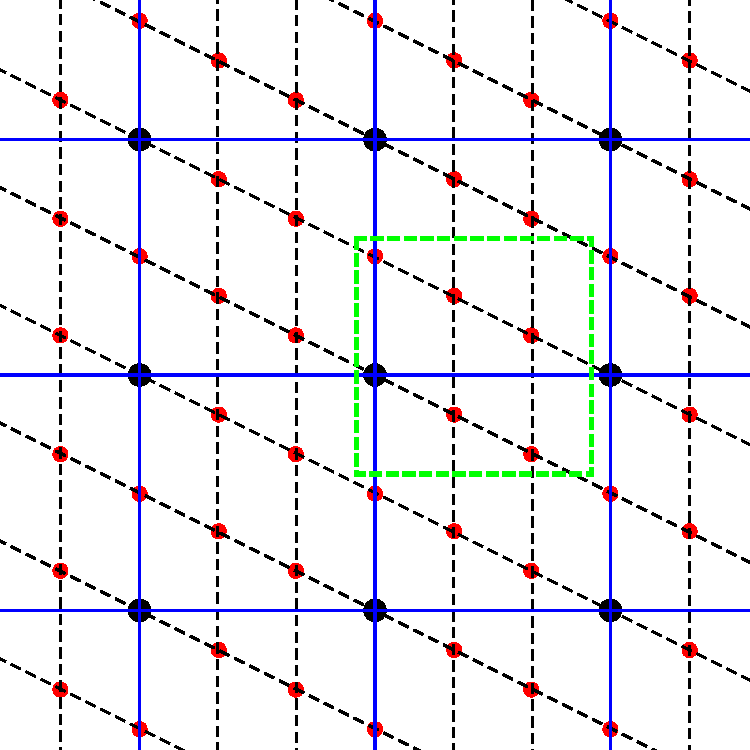
\includegraphics[width=0.40\textwidth]{HLReciprocalLattice2}
  \caption{\label{fig:HLReciprocalLattice2}
(Color online)
The reciprocal lattices of both the Bravais lattice $\Lambda$ and the
integer square lattice. The red points are the reciprocal lattice $\Lambda^*$ of the Bravais
lattice $\Lambda$ in \reffig{fig:BravaisLatt}. The black points are
the reciprocal lattice of the square lattice. Each of these squares
enclosed by the blue lines has edge length $2 \pi$.
%And these squares are also repeating unit of the wave vectors (the red dots in this figure).
Two wave vectors are equivalent if they are different by a
reciprocal lattice vector of the square lattice.
}
\end{figure}
%%%%%%%%%%%%%%%%%%%%%%%%%%%%%%%%%%%%%%%%%%%%%%%%%%%%%%%%%%%%%%%



\subsection{Backup from s previous version of \catlatt}

The set of all wave vectors $\mathbf{K}_m$ that yield plane waves with
the periodicity of a given Bravais lattice defines its reciprocal
lattice. The $\mathbf{K}_m$ are called reciprocal lattice vectors.

% from Barvinok \arXiv{/math/0504444}:
Let $\langle \cdot, \cdot \rangle$ be the scalar product on $\reals^d$.
% and the corresponding Euclidean norm $\| \cdot\|$.
Let $\Lambda \subset\reals^d$ be a lattice,
and let  $\Lambda^{\ast} \subset\reals^d$ be its {\it reciprocal} lattice
\beq
\Lambda^{\ast}=
\Bigl\{x \in \reals^d: \quad \langle x, y \rangle \in {\Bbb Z} \quad
\mbox{for all} \quad y \in \Lambda
\Bigr\}\,.
\ee{dualLatt}

The reciprocal lattice of the Bravais lattice \refeq{2DBravaisLattice} is
spanned by reciprocal basis \refeq{RecLattBasis}
\beq
\Lambda^* = \{n_1 \mathbf{b}_1 + n_2 \mathbf{b}_2\,|\,n_i \in \mathbb{Z}\}
\,.
\ee{2DReciprocalLattice}
The eigenvectors of the translation operator have the form
of a plane wave
\beq
f_{k}({z})
= e^{i {k} \cdot {z}} \, , \quad {k} \in \Lambda^*
\,,
\ee{2DEigenvectors}
and, in addition, satisfy the Bravais lattice \refeq{2DBravaisLattice}
periodicity.



Then the basis vectors of the reciprocal lattice are:
\beq
\left[
\begin{array}{cc}
\mathbf{b}_1 & \mathbf{b}_2 \\
\end{array}
\right]
=
\frac{2 \pi}{\speriod{} \period{}}
\left[
\begin{array}{cc}
 \period{} & 0 \\
 -{S} & \speriod{} \\
\end{array}
\right]
 \, .
\ee{2DReciprocalBasis}
A plane wave with wave vector $\mathbf{k}$ in
the reciprocal lattice $\Lambda^*$ is an eigenvector of the
{\jacobianOrb} \refeq{dDCatsT} that satisfies the periodic condition of
Bravais lattice $\Lambda$. The eigenvector with wave vector
$\mathbf{k}=n_1\mathbf{b}_1+n_2\mathbf{b}_2$ is
\beq
f_{k}({z}) = e^{i {k} \cdot {z}}
  = \exp\left(
      i\frac{2 \pi}{\speriod{} \period{}}(n_1 \period{} z_1 - n_1 {S} z_2 + n_2 \speriod{} z_2)
        \right)
\,,
\ee{2DEigenvector}
where the ${z}=(z_1,z_2)$, with the {\jacobianOrb}  eigenvalue
\beq
\lambda_{k}
= \sum_{j=1}^2 ({s} - 2 \cos k_j)
= 2s - 2 \cos2\pi(\frac{n_1}{\speriod{}})
    - 2 \cos2\pi(\frac{n_1 {S}}{\speriod{} \period{}}
                -\frac{n_2}{\period{}})
\,.
\ee{2DEigenvalue}
As the field has support on the square lattice sites, it suffices to use
the wave vectors
$\mathbf{k}= n_1 \mathbf{b}_1 + n_2 \mathbf{b}_2$
with $n_1$ from 0 to $\speriod{}-1$ and $n_2$ from 0 to $\period{}-1$ to
get all the reciprocal lattice eigenvectors.
    \PC{2020-05-28}{Perhaps use
\[
\cos(a-b) = \cos(a)\cos(b) + \sin(a)\sin(b)
\,?
\]
\[
\cos(2a) = \cos(a)^2 - \sin(a)^2 = 1 - 2\sin(a)^2
\,?
\]
\[
{s}-2\cos k_1  = ({s}-2) + 4(\sin(k_1/2))^2
\]
\[
{s}-2\cos k_2  = ({s}-2) + 4(\sin(k_1/2))^2
\]
Set \(q_1=2\pi{k_1}/{\speriod{}}\,,\)
\(q_2=2\pi{k_2}/{\period{}}\,,\)
\(C=\speriod{}/{\period{}}\,,\)
\[
2\cos(q_2-Cq_1) = 2\cos(q_2)\cos(Cq_1) + 2\sin(q_2)\sin(Cq_1)
\]
    }

This range contains all of the wave vectors in one lattice cell of
reciprocal lattice of the square lattice, as shown in
\reffig{fig:HLReciprocalLattice2}, where wave vectors with $n_1$ from 0
to $\speriod{}-1$, and $n_2$ from 0 to $\period{}-1$ are enclosed by the
green dashed square. Any wave vector on the reciprocal lattice
$\Lambda^*$ outside of this range will give an eigenvector which is
equivalent to an eigenvector with the wave vector within this range. So
the number of eigenvectors is $\speriod{} \period{}$, which is the number
of square lattice sites within the minimal repeating tile.

The 4-index {\jacobianOrb} \refeq{dDCatsT} is a matrix with indices in a
finite range. The {\jacobianOrb} has $\speriod{}\period{}$ eigenmodes. We
know that the number of {\twots} is equal to the {\HillDet} of the
{\jacobianOrb}, which is the product of all the eigenvalues,
% $N_{\LTS{}{}{}}=\prod_{k}\lambda_{k}$,
\beq
N_{\LTS{}{}{}}
=  2^{\speriod{}\period{}}\prod_{k_1=0}^{\speriod{}-1} \prod_{k_2=0}^{\period{}-1}
     \left[s  -  \cos\left(\frac{2\pi k_1}{\speriod{}}\right)
              -  \cos\left(
                            \frac{2\pi k_2}{\period{}}
                           -\frac{2\pi k_1}{\speriod{}}
                            \frac{ \tilt{}}{\period{}}
                     \right)
     \right]
%.
\label{2DCountingFormula}
\eeq

Given the eigenmodes with a given periodic condition, one can reduce the
2\dmn\ square lattice to a finite repeating tile. The {\sPe} in this tile
is still \refeq{dDCatsT}. But now the fields and sources are defined over an
$\LTS{}{}{}$ lattice.

\beq
N_{\BravCell{1}{1}{0}} =  2s - 4 = 1
 \,.
\label{1x1DCount}
\eeq

\beq
N_{\BravCell{\speriod{}}{1}{0}}
=  \prod_{k_1=0}^{\speriod{}-1}
     \left[2s_2 - 2 - 2 \cos\left(\frac{2\pi k_1}{\speriod{}}\right)
     \right]
 \,.
\label{2Dto1DCount}
\eeq
Comparing with the \templatt\ count \refeq{appe:detTemCatCheb} we see
that the count is the same, provided we replace
\(
{s}_1\to2({s}_2-1)
\,,
\)
in agreement with the 3-term recurrence \refeq{eq:CatLattT=1}.


\subsubsection{$\BravCell{2}{1}{1}$ \twots.}
\label{s:catLatt2x2rel1}
%    \HLpost{2019-11-22}{
For $s=5/2$ \catlatt.
\beq
N_{\BravCell{2}{1}{1}}
= \prod_{l=0}^{1}
  \Big[
  2s - 4 \cos2\pi\left(\frac{l}{2}\right)
  \Big]
= 9
 \,.
\ee{2x1_1Fourier}

\subsubsection{$\BravCell{2}{2}{0}$ \twots.}
\label{s:catLatt2x2}
For $s=5/2$ \catlatt.
\[
N_{[2\!\times\!2]} =
2^4({s}- 2)({s}- \cos\pi -1)({s}- 1 - \cos\pi)({s}- \cos\pi - \cos\pi) = 225
\,.
\]

\subsubsection{$\BravCell{3}{2}{0}$ \twots.}
\label{s:catLattRel3x2}
%    \HLpost{2019-11-23}{
For $s=5/2$ only 850 prime $\BravCell{3}{2}{0}$ \brick s are \admissible. The
integer points count \refeq{HL[3x2]count} is in agreement with the
counting formula \refeq{2DCountingFormula} for the $\BravCell{3}{2}{0}$
\twots:
     \[
N_{\BravCell{3}{2}{0}}
  = \prod_{l=0}^2\prod_{t=0}^1\left[
  2{s}-2\cos\left(\frac{2 \pi l}{3}\right)-2\cos\left(\frac{2 \pi t}{2}\right)
                              \right]
  = 5120
     \,.
     \]

%%%%%%%%%%%%%%%%%%%%%%%%%%%%%%%%%%%%%%%%%%%%%%%%%%%%%%%%%%%%%%%%%%%%%%%
\renewcommand{\statesp}{phase space}
\renewcommand{\Statesp}{Phase space}
\renewcommand{\stateDsp}{phase-space}
\renewcommand{\StateDsp}{Phase-space}
